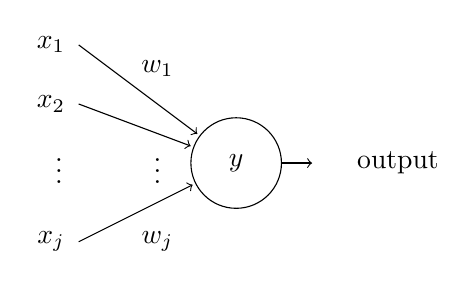
\begin{tikzpicture}[shorten >=1pt,->]
		\tikzstyle{unit}=[draw,shape=circle,minimum size=1.15cm]
 
		\node[unit](p) at (2,1){$y$};
		\node(dots) at (-0.25,1){\vdots};
		\node(dots2) at (1,1){\vdots};
		\node(w1) at (1.0,2.2){$w_1$};
		\node(wj) at (1.0,0){$w_j$};
 
		\draw (0,2.5) node[xshift=-10]{$x_1$} -- (p);
		\draw (0,1.75) node[xshift=-10]{$x_2$} --(p);
		\draw (0,0) node[xshift=-10]{$x_j$} -- (p);
		\draw (p) -- (3,1) node[xshift=30]{output};
% 		\draw (1.2,2.2) node[xshift=-10]{$w_1$};
	\end{tikzpicture}